\chapter{Nombres relatifs}\label{ChNbRelatifs}
\begin{acquis}
\begin{itemize}
\item donner le signe d'un nombre relatif;
\item déterminer l'opposé d'un nombre relatif;
\item lire l'abscisse d'un point sur une droite graduée;
\item placer un point dont je connais l'abscisse sur une droite graduée;
\item donner la valeur absolue d'un nombre;
\item lire les coordonnées d'un point dans un repère;
\item placer un point dont je connais les coordonnées dans un repère;
\item comparer deux nombres relatifs de même signe ou de signes différents.
\end{itemize}
\end{acquis}

\activites

\begin{activite}[De nouveaux nombres]

\begin{partie}[1\up{ère} approche]
 \begin{enumerate}
  \item Trace une demi-droite graduée d'origine le point $O$ en prenant le centimètre comme unité. Place les points $A(3)$, $B(4)$ et $D(9)$.
  \item Construis le point $C$ tel que $A$ soit le milieu du segment $[BC]$. Quelle est l'abscisse du point $C$ ?
  \item On veut placer le point $E$ tel que $A$ soit le milieu du segment $[DE]$. Que constates-tu ? Comment compléter cette graduation pour résoudre complètement ce problème ? Quelle est alors l'abscisse du point $E$ ?
  \end{enumerate}
\end{partie}

\begin{partie}[2\up{ème} approche]
 \begin{minipage}[t]{0.40\linewidth}
Ce matin, il faisait très froid. La température a augmenté de \textcolor{H1}{$5^\circ$C}, il fait maintenant $3^\circ$C.
 
 Pour trouver la température de ce matin, nous allons tester différentes valeurs. Recopie puis complète le tableau ci-contre :
 
  \end{minipage} \hfill%
  \begin{minipage}[t]{0.56\linewidth}
  \centering
  
\includegraphics[width=1.9cm]{5}
  
  \begin{tabularx}{0.8\linewidth}{|X|X|}
   \hline
   \rowcolor{J2} Température du matin & Température actuelle \\\hline
   \rowcolor{J2} 5 & \\\hline
   \rowcolor{J2} 3 & \\\hline
   \rowcolor{J2} 1 & \\\hline
   \rowcolor{J2} 0 & \\\hline
   \end{tabularx}
   \end{minipage} \\
   
  \begin{enumerate}
  \item Les différentes valeurs testées répondent-elles au problème ? En conséquence, la température du matin peut-elle être supérieure à 0 ?
  \item Quelle était alors la température ce matin ?
  \end{enumerate}
\end{partie}

\begin{partie}[Utilisation de ces nouveaux nombres]
Dans quelles circonstances de la vie quotidienne as-tu rencontré des nombres possédant un signe $+$ ou $-$ ? Donne des exemples en histoire, en physique ou dans d'autres domaines. 
\end{partie}

\end{activite}

%%%%%%%%%%%%%%%%%%%%%%%%%%%%%%%%%%%%%%%%%%%%%%%%%%%%%%%%%%%%%%%%%%%%%%

\begin{activite}[Opposés ?]

\begin{enumerate}
 \item Trace une droite graduée d'origine $O$ en prenant le centimètre comme unité.
 \item Place les points $A$ et $C$ d'abscisses respectives $+ 3$ et $- 6$.
 \item Place :
 \begin{itemize}
  \item Le point $B$ tel que $O$ soit le milieu du segment $[AB]$ ;
  \item Le point $D$ tel que $O$ soit le milieu du segment $[CD]$.
  \end{itemize}
 \item Reproduis et complète le tableau ci-dessous : \\[1em]
  \begin{tabularx}{\linewidth}{|c|X|X|X|X|}
   \hline
   \rowcolor{J2} Point & A & B & C & D \\\hline
   \rowcolor{J2} Abscisse du point & $+ 3$ & & $- 6$ & \\\hline
   \rowcolor{J2} Distance du point à l'origine $O$ (en centimètres) & & & & \\\hline
   \end{tabularx} \\[1em]
  On dit que : « La \textbf{valeur absolue} d'un nombre relatif correspond à la distance entre l'origine O et le point qui a pour abscisse ce nombre ». 

 \item Donne la valeur absolue des nombres relatifs suivants : $+ 7$ ; $- 4$ ; $- 6,2$ ; $+ 17,8$.
 \item Donne deux nombres différents qui ont la même valeur absolue. Que constates-tu ? Quel adjectif peux-tu utiliser pour qualifier ces deux nombres ?
 \end{enumerate}
 
\end{activite}

%%%%%%%%%%%%%%%%%%%%%%%%%%%%%%%%%%%%%%%%%%%%%%%%%%%%%%%%%%%%%%%%%%%%%%

\begin{activite}[Manque de repères ?]

On a dessiné un repère du plan sur une carte de Suisse. L'origine de ce repère est la ville de Kerns dans le canton d'Obwald, représentée par le point $O$. \scriptsize{(source de la carte de Suisse : Pymouss, Wikipedia)}

\begin{center} \includegraphics[width=13cm]{carteCH} \end{center}
\normalsize{Le professeur propose de chercher les coordonnées de Locarno qui permettent de la situer par rapport au point $O$ dans ce repère. Voici les réponses de trois élèves de la classe :}
\begin{itemize}
 \item Dylan dit : « Les coordonnées de Locarno, c'est $+ 20$ » ;
 \item Julia dit : « Les coordonnées de Locarno sont d'abord $+ 20$ puis $- 34$ » ;
 \item Medhi dit : « Les coordonnées de Locarno sont d'abord $- 34$ puis $+ 20$ ».
 \end{itemize}
 \begin{enumerate}
  \item Dylan a-t-il donné suffisamment d'informations pour repérer la ville de Locarno ? Dans un repère du plan, combien de nombres sont nécessaires pour repérer un point ?
  \item Les réponses de Julia et Medhi manquent de précision. Pourquoi ? Réécris celles-ci afin qu'elles soient complètes. \\[1em]
Pour écrire les coordonnées d'un point, on écrit d'abord le nombre qui se lit sur l'axe horizontal puis le nombre qui se lit sur l'axe vertical, en les mettant entre parenthèses et en les séparant par un point-virgule.
  \item Écris les coordonnées de Genève, Lausanne, Neuchâtel, Zürich, Fribourg et Poschiavo.
  \item Donne le nom des villes dont les coordonnées sont : $(+ 45 ; 0)$ ; $(+ 40 ; + 31)$ ;  $(- 27 ; + 9)$ et $(- 35 ; - 32)$.
  \item Quand on va d'Ouest en Est, que remarques-tu concernant le premier nombre des coordonnées ? Quand on va du Nord vers le Sud, que remarques-tu concernant le deuxième nombre des coordonnées ?
  \item Fabien donne les coordonnées d'une ville du quart Nord-Est : $(- 13 ; + 32)$. Luciana lui dit qu'il y a forcément une erreur. Pourquoi ? Corrige l'erreur de Fabien et cite la ville dont il voulait parler.
  \end{enumerate}
  
\end{activite}

%%%%%%%%%%%%%%%%%%%%%%%%%%%%%%%%%%%%%%%%%%%%%%%%%%%%%%%%%%%%%%%%%%%%%%

\begin{activite}[Comparaison de nombres relatifs]
Sur l'axe gradué ci-dessous, on a placé les points $A$ à $H$.

\begin{center} 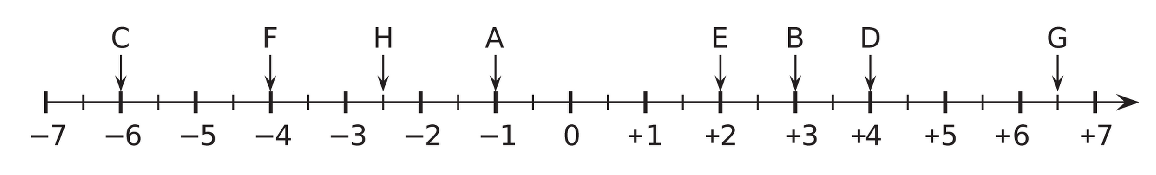
\includegraphics[width=14cm]{axe} \end{center}

 \begin{enumerate}
  \item Lorsqu'on parcourt l'axe gradué de gauche à droite, comment sont rangées les abscisses des points ? Donne les abscisses des points $A$ à $F$ et celles de $G$ et $H$.
  \item En observant l'axe gradué, recopie en remplaçant les .... par $<$ ou $>$ :
   \begin{colitemize}{3}
    \item $- 6 \ldots  \ldots - 1$ ;
    \item $+ 3 \ldots  \ldots - 6$ ;
    \item $+ 4 \ldots  \ldots - 6$ ;
    \item $- 1 \ldots  \ldots + 2$ ;
    \item $+ 2 \ldots  \ldots + 4$ ;
    \item $+ 4 \ldots  \ldots + 3$ ;
    \item $- 1 \ldots  \ldots - 4$ ;
    \item $- 4 \ldots  \ldots - 6$ ;
    \item $- 2,5 \ldots  \ldots + 6,5$.
    \end{colitemize}
  \item Entoure en rouge les cas pour lesquels tu as comparé deux nombres positifs. Observe ces cas et déduis-en une règle qui permet de comparer deux nombres positifs. Tu utiliseras l'expression « valeur absolue » pour rédiger cette règle. 
  \item Entoure en bleu les cas pour lesquels tu as comparé un nombre positif et un nombre négatif. Observe ces cas et déduis-en une règle qui permet de comparer un nombre positif et un nombre négatif.
  \item Entoure en vert les cas pour lesquels tu as comparé deux nombres négatifs. Observe ces cas et déduis-en une règle qui permet de comparer deux nombres négatifs. Tu utiliseras l'expression « distance à zéro » pour rédiger cette règle.
  \end{enumerate}
  
\end{activite}



\cours
\prof
Dans ce cours, on prendra soin de faire le lien avec les ensembles de nombres. Faire un rappel grâce que schéma donné au début de cet ouvrage.

\section{Les nombres relatifs}

% remarque : pour qu'un mot se retrouve dans le lexique : \MotDefinition{asymptote horizontale}{} 

\vspace{4em}

\begin{center}
    \begin{tikzpicture}[every node/.style={scale=0.6}]



%contour immeuble
\draw[fill=gray!40!yellow] (0,-3) rectangle (4,6);
%cage ascenseur
\draw[fill=gray!20] (1.5,-3)rectangle (2.5,6);
%étages sous-sol
\foreach \y in {-2,-1,1}{\draw (0,\y)--(1.5,\y) (2.5,\y)--(4,\y);}
%rez de chaussée (couleur différente)
\draw[fill=yellow!30!white] (0,0) rectangle (1.5,1) (2.5,0) rectangle (4,1); 
%niveau du sol
\draw[fill=gray!80] (-1,0) rectangle (5,0.1);
%fenêtres étages
\foreach \y in {1,2,...,5}{\foreach \x in {0.3,0.9,2.8,3.4} {\draw[fill=blue!40] (\x,\y+0.2) rectangle (\x+0.3,\y+0.8);}}
%ascenseur
\draw[fill=white] (1.6,2) rectangle (2.4,3);
\draw (2.2,5.7) circle (2mm);
\draw[very thick](2,3)--(2,5.7);
\draw[very thick] (2,5.7) arc (180:-80:2mm);
%boutons ascenseur étages
\foreach \y in {1,2,...,5}{\node[draw,circle,minimum size=1cm,fill=H2,text=black,scale=1] at (5.5,\y+0.5){\y}; }
\node[draw,circle,minimum size=1cm,fill=A2,text=black,scale=1] at (5.5,0.5){0}; 
\node[minimum width=1.5cm,minimum height=1cm,rounded corners=4pt,draw,rectangle,fill=A2,text=black,scale=1] at (7,0.5){Rez de chaussée}; 
\foreach \y in {-1,-2,-3}{\node[minimum width=1cm,minimum height=1cm,rounded corners=4pt,draw,rectangle,fill=B2,text=black,scale=1] at (5.5,\y+0.5){\y}; }

%insertion personnages
\draw (1.8,2.3) node[santa,minimum size=0.6cm]{} ;
\draw (2.2,2.3) node[mexican,minimum size=0.6cm]{} ;
%\draw (4,0) node[duck,minimum size=1.5cm]{};


\end{tikzpicture}
\end{center}

\begin{definition}
Lorsqu'on effectue un déplacement, deux données sont importantes:
\begin{itemize}
    \item le sens du déplacement
    \item la longueur du déplacement
\end{itemize}

En mathématiques, ce déplacement est caractérisé par \textcolor{C2}{\textbf{un nombre relatif}}.\\
\end{definition}

%%%%%%%%%%%%%%%%%%%%%%%%%%%%%%%%%%%%%%%%%%%%%%%%%%%%%%%%%%%%%%%%%
\begin{definition}
On commence toujours à compter à partir de 0.\\
Lorsque que le nombre est \textbf{inférieur à 0} (à gauche ou en dessous de 0), on parle de \textcolor{C2}{\textbf{nombre négatif}} et on utilise un signe $-$ placé devant le chiffre.\\
Lorsque que le nombre est \textbf{supérieur à 0} (à droite ou en dessus de 0), on parle de \textcolor{C2}{\textbf{nombre positif}} et on peut alors utiliser un signe $+$ placé devant le chiffre mais ce n'est pas toujours obligatoire.\\
0 est le seul nombre à la fois positif et négatif.\\
\end{definition}



%%%%%%%%%%%%%%%%%%%%%%%%%%%%%%%%%%%%%%%%%%%%%%%%%%%%%%%%%%%%%%%%%
\begin{definition}
La valeur du déplacement est donnée par le chiffre placé après le signe. C'est ce qu'on appelle \textcolor{C2}{\textbf{ la valeur absolue}}.
Il s'agit de la distance entre 0 est le nombre relatif. Il existe une notation pour parler de la valeur absolue:|nombre|\\
Deux nombres relatifs qui ne diffèrent \textbf{que} par leur signe sont \textcolor{C2}{\textbf{opposés}}.
\end{definition}

\begin{methode*1}[Trouver la valeur absolue d'un nombre relatif]


\begin{exemple*1}
Donne la valeur absolue du nombre $-2$ :

$|-2|$ = 2.
\end{exemple*1}


\exercice
Donne la valeur absolue des nombres suivants : $+5$ ; $-7$ ; $+64,78$ et $-123,4$.
%\correction

\end{methode*1}


\begin{methode*1}[Savoir utiliser le vocabulaire]



\begin{exemple*1}
Quel est le signe du nombre $-3$ ? Quel est son opposé ? \\[1em]
Le signe de $- 3$ est $-$, il est négatif. Son opposé est $+ 3$ que l'on écrit aussi 3.
\end{exemple*1}

\exercice 
Donne le signe des nombres relatifs suivants :

$+1235$ ; $-587$ ; $0$ ; $-1$ ;  $3,5$ ; $-0,001$.
%\correction

\exercice 
Donne l'opposé des nombres relatifs suivants :

$-2,531$ ; $0$ ; $1,245$ ;  $-0,03$ et $0,003$.
%\correction

\end{methode*1}



%%%%%%%%%%%%%%%%%%%%%%%%%%%%%%%%%%%%%%%%%%%%%%%%%%%%%%%%%%%%%%%%%

\newpage


\begin{aconnaitre}
Tout point d'une droite graduée est repéré par un nombre relatif appelé son \textcolor{C2}{\textbf{abscisse}}.

\begin{tikzpicture}
\draw[->] (-6,0) -- (6,0);
\draw (0,.2) node[above] {$O$} ;
\draw (0,-.2) node[below] {$0$} ;
\draw (1,-.2) node[below] {$+1$} ;
\draw (-4,1) node {$A$} ;
\draw[->] (-4,.8) -- (-4,.2) ;
\draw (0,0) node {$|$} ; \draw (1,0) node {$|$} ; \draw (2,0) node {$|$} ; \draw (3,0) node {$|$} ; \draw (4,0) node {$|$} ; \draw (5,0) node {$|$} ;
\draw (-1,0) node {$|$} ; \draw (-2,0) node {$|$} ; \draw (-3,0) node {$|$} ; \draw (-4,0) node {$|$} ; \draw (-5,0) node {$|$} ;
\end{tikzpicture}

\end{aconnaitre}

\vspace{2em}


\begin{methode*1}[Repérer un point sur une droite graduée]



\begin{exemple*1}
Sur la droite graduée ci-dessus, lis l'abscisse du point $A$ : \\[1em]
\begin{minipage}[c]{0.4\linewidth}
Le point $A$ est à gauche de l'origine :

son abscisse est donc négative.

La distance du point $A$ au point $O$ est $4$.
 \end{minipage} \hfill%
 \begin{minipage}[c]{0.1\linewidth}
 \begin{center}
\includegraphics[width=0.23cm]{accolade_droite}\end{center}
  \end{minipage} \hfill%
  \begin{minipage}[c]{0.4\linewidth}
  donc l'abscisse du point $A$ est $-4$.
   \end{minipage} \\
\end{exemple*1}


\begin{exemple*1}
Trace une droite graduée et place les points $B(+6)$ et $C(-5)$ : \\[1em]
\begin{minipage}[c]{0.4\linewidth}
L'abscisse du point $B$ est $+6$ donc
 \end{minipage} \hfill%
 \begin{minipage}[c]{0.1\linewidth}
 \begin{center}
\includegraphics[width=0.23cm]{accolade_gauche}\end{center}
  \end{minipage} \hfill%
  \begin{minipage}[c]{0.4\linewidth}
  Son abscisse est positive : le point $B$ est donc à droite de l'origine.
  
  Sa distance à l'origine est de 6 unités.
  \end{minipage} \\[0.5em]

\begin{minipage}[c]{0.4\linewidth}
L'abscisse du point $C$ est $-5$ donc
 \end{minipage} \hfill%
 \begin{minipage}[c]{0.1\linewidth}
 \begin{center}
\includegraphics[width=0.23cm]{accolade_gauche}\end{center}
  \end{minipage} \hfill%
  \begin{minipage}[c]{0.4\linewidth}
  Son abscisse est négative : le point $C$ est donc à gauche de l'origine. 
  
  Sa distance à l'origine est de 5 unités.
   \end{minipage} \\

\begin{tikzpicture}
\draw[->] (-5.5,0) -- (6.5,0);
\draw (0,.2) node[above] {$O$} ;
\draw (0,-.2) node[below] {$0$} ;
\draw (1,-.2) node[below] {$+1$} ;
\draw (-5,1) node {$C$} ; \draw[->] (-5,.8) -- (-5,.2) ;
\draw (6,1) node {$B$} ; \draw[->] (6,.8) -- (6,.2) ;
\draw (0,0) node {$|$} ; \draw (1,0) node {$|$} ; \draw (2,0) node {$|$} ; \draw (3,0) node {$|$} ; \draw (4,0) node {$|$} ; \draw (5,0) node {$|$} ;\draw (6,0) node {$|$} ;
\draw (-1,0) node {$|$} ; \draw (-2,0) node {$|$} ; \draw (-3,0) node {$|$} ; \draw (-4,0) node {$|$} ; \draw (-5,0) node {$|$} ;
\end{tikzpicture}

\end{exemple*1}


\exercice
Trace une droite graduée d'origine $O$, une unité valant 2 cm. Places-y les points $A$, $B$, $C$, $D$ et  $E$, $F$ d'abscisses respectives $+3$ ; $-2$ ; $+5$ ; $-3$ et $-1,5$ ; $+2,5$. Que peux-tu dire des abscisses de $A$ et $D$ ?
%\correction

\end{methode*1}

%%%%%%%%%%%%%%%%%%%%%%%%%%%%%%%%%%%%%%%%%%%%%%%%%%%%%%%%%%%%%%%%

\section{Comparaison}

\vspace{4em}

\begin{aconnaitre}
\MotDefinition{Comparer deux nombres}{}, c'est trouver lequel est le plus grand (ou le plus petit) ou dire s'ils sont égaux.
\end{aconnaitre}

\vspace{4em}

\begin{methode*1}[Comparer deux nombres relatifs]


\begin{exemple*1}
Compare 9,37 et 92,751 puis 81,36 et 81,357 :

On compare d'abord les \textbf{\textcolor{H1}{parties entières}} des deux nombres :
\begin{itemize}
 \item $\textbf{\textcolor{H1}{9}} < \textbf{\textcolor{H1}{92}}$ donc $9,37 < 92,751$.
 \item $81,357$ et $81,36$ ont la même partie entière. On compare alors les \textbf{\textcolor{B2}{parties décimales}} : $81,357 = 81+0,357$ et $81,36=81+0,36$ mais $0,36=0,360$.
 \end{itemize}
Or \textbf{\textcolor{B2}{360 millièmes}} est plus grand que \textbf{\textcolor{B2}{357 millièmes}} donc $81,36 > 81,357$.
\end{exemple*1}


\begin{exemple*1}
Écris un encadrement de 1,564 au dixième : \\[0.5em]
$1,564 = 1 + 0,500 + 0,064$ et 0,064 est plus petit que 1 dixième. Ainsi, 1,564 est compris entre $1 + 0,5$ et $1 + 0,5 + 0,1$ , soit $1 + 0,6$. \\[0.5em]
Donc un encadrement au dixième de 1,564 est : $1,5 < 1,564 < 1,6$.
\end{exemple*1}

\exercice
Compare les nombres suivants :
\begin{colenumerate}{3}
 \item $+5$ et $+9$ ;
 \item $-3$ et $+8$ ;
 \item $-6$ et $-12$ ;
 \item $-5$ et $-9$ ;
 \item $5,1$ et $-5,3$ ;
 \item $-6,2$ et $-6,4$.
 \end{colenumerate}
%\correction

\end{methode*1}


\newpage

\begin{aconnaitre}
\textbf{Deux nombres relatifs positifs} sont rangés dans l'ordre de leur valeur absolue.

Un \textbf{nombre relatif négatif} est inférieur à un \textbf{nombre relatif positif}.

\textbf{Deux nombres relatifs négatifs} sont rangés dans l'ordre inverse de leur valeur absolue.
\end{aconnaitre}

\vspace{4em}


\begin{methode*1}[Comparer des nombres relatifs]

\begin{exemple*1}
Compare les nombres $-9$ et $-7$ : \\[0.5em]
\begin{tabular}{ccl} 
 $-9$ et $-7$ & $\longrightarrow$ & On veut comparer deux nombres relatifs négatifs. \\
 $9 > 7$ & $\longrightarrow$ & On détermine les valeurs absolues de $-9$ et de $-7$ puis  \\
& & on les compare. \\
 $-9 < -7$ & $\longrightarrow$ & On range les nombres $-9$ et $-7$ dans l'ordre inverse de leur  \\
 & & valeur absolue. \\
 \end{tabular}
\end{exemple*1}


\exercice
Range dans l'ordre croissant les nombres suivants : 
\begin{colenumerate}{2}
 \item $+12$ ; 0 ; $-7$ ; $-5$ ; $+5$ ;
 \item $-8$ ; $+10$ ; $-14$ ; $-21$ ; $+3$ ; $-1$ ;
 \item $-24$ ; $-2,4$ ; $2,4$ ; 0 ; $-4,2$ ; $-4$ ;
 \item $-2,4$ ; $+2,3$ ; $-2,42$ ; $+2,33$ ; $-3,23$.
 \end{colenumerate}
%\correction

\end{methode*1}
%%%%%%%%%%%%%%%%%%%%%%%%%%%%%%%%%%%%%%%%%%%%%%%%%%%%%%%%%%%%%%%%%
\newpage


\section{Repérage dans un plan}

\vspace{3em}

\begin{definition}
Dans un plan muni d'un repère, tout point est repéré par un couple de nombres relatifs appelé ses \MotDefinition{coordonnées}{} : la première est l'\textcolor{C2}{\textbf{abscisse}} (déplacement horizontal) et la seconde est l'\textcolor{C2}{\textbf{ordonnée}} (déplacement vertical).\\
Pour un point A, on écrira toujours \textbf{A(abscisse de A ; ordonnée de A)}.
\end{definition}

\vspace{3em}

\begin{methode*1}[Repérer un point dans un plan]

\begin{exemple*1}
Lis les coordonnées du point $A$ et du point $B$ puis place les points $C(5 ; -3)$ et $D(-3 ; 0)$ :

\begin{center} 
\begin{tikzpicture}[general,scale=0.5]
\draw[xstep=1,ystep=1,color=gray!80] (-6,-4) grid (6,4);
\axeX{-6}{6}{1}
\axeY{-4}{4}{1}

\draw[ultra thick,loosely dotted,color=C1](-4,2)--(0,2);
\node[right,color=C1,font=\bfseries] at (0,2){$+2$};
\draw[ultra thick,loosely dotted,color=G1](-4,2)--(-4,0);
\node[below,color=G1,font=\bfseries] at (-4,0){$-4$};

\node at (0,-3){$\bullet$};
\node[above left,font=\bfseries] at (-4,2){A};
\node at (-4,2){$\bullet$};
\node[right,font=\bfseries] at (0,-3){B};
\end{tikzpicture}
\end{center}

Pour lire les coordonnées du point $A$, on repère l'abscisse de $A$ sur l'axe horizontal (pointillés bleus) puis  son ordonnée sur l'axe vertical (pointillés violets). On conclut en donnant l'abscisse puis l'ordonnée : $A (-4 ; +2)$. \\[0.5em]
Le point $B$ appartient à l'axe des ordonnées donc son abscisse est 0. Ses coordonnées sont $(0 ; -3)$.

Pour placer le point $C$, on repère tous les points d'abscisse $+5$ puis on repère tous les points d'ordonnée $-3$. On place le point $C$ à l'intersection des deux lignes. \\[0.5em]
L'ordonnée du point $D$ est 0 donc $D$ appartient à l'axe des abscisses.
\end{exemple*1}

\exercice 

\begin{minipage}[c]{0.45\linewidth}
Sur la figure ci-contre, lis les coordonnées des points $K$, $L$, $M$, $N$, $P$ et $R$ :
 \end{minipage} \hfill%
 \begin{minipage}[c]{0.4\linewidth}
 \begin{center} 
\begin{tikzpicture}[general,scale=0.5]
\draw[xstep=1,ystep=1,color=gray!80] (-6,-4) grid (6,3);
\axeX{-6}{6}{1}
\axeY{-4}{3}{1}

\node at (-3,2){$\bullet$};
\node[left,font=\bfseries] at (-3,2){K};
\node at (-5,0){$\bullet$};
\node[below,font=\bfseries] at (-5,0){L};
\node at (2,-3){$\bullet$};
\node[left,font=\bfseries] at (2,-3){M};
\node at (0,1){$\bullet$};
\node[right,font=\bfseries] at (0,1){N};
\node at (4,-1){$\bullet$};
\node[left,font=\bfseries] at (4,-1){P};
\node at (-4,-3){$\bullet$};
\node[left,font=\bfseries] at (-4,-3){R};
\end{tikzpicture}
\end{center}
  \end{minipage} \\
%\correction

\exercice Trace sur ton cahier un repère d'origine $O$. L'unité de longueur est le centimètre sur les deux axes. Place les points suivants :
\begin{colenumerate}{4}
 \item $E(+2 ; +3)$ ;
 \item $F(-2 ; -3)$ ;
 \item $G(+2 ; -3)$ ;
 \item $H(-2 ; 3)$.
 \end{colenumerate}
%\correction

\end{methode*1}






\exercicesbase
\begin{colonne*exercice}

\serie{Vocabulaire}

\begin{exercice}[Dans la vie courante]
Donne des exemples de la vie courante pour lesquels on utilise :
\begin{enumerate}
 \item Des nombres entiers relatifs ;
 \item Des nombres relatifs non nécessairement entiers.
 \end{enumerate}
\end{exercice}


\begin{exercice}[Interprétation]
Parmi la liste de mots suivants, quels sont ceux qui peuvent «se traduire» à l'aide : 
\begin{enumerate}
 \item D'un nombre relatif positif ?
 \item D'un nombre relatif négatif ?
 \item Du nombre relatif «0» ?
 \end{enumerate}
 
Diminuer, croître, soldes, monter, croissance, recul, freiner, augmenter, déclin, progression, ajouter, hausse, maigrir, ôter, dépense, régression, stable, descendre, accélérer, baisse, centupler, fixe, atténuer, constant, restreindre, chute, ascendant, amoindrir, stagnation.
\end{exercice}


\begin{exercice}
Recopie et complète les phrases en utilisant les mots proposés :

\boxed{\text{positif}} \quad \boxed{\text{négatif}} \quad \boxed{\text{plus}} \quad \boxed{\text{relatif}} \quad \boxed{\text{opposé}}

\begin{enumerate}
 \item $-4$ est un nombre \ldots \ldots \ldots \ldots ;
 \item Un nombre \ldots \ldots \ldots \ldots peut s'écrire sans le signe \ldots \ldots \ldots \ldots ;
 \item L' \ldots \ldots \ldots \ldots d'un nombre relatif \ldots \ldots \ldots \ldots est un nombre relatif \ldots \ldots \ldots \ldots ;
 \item $+3$ est l' \ldots \ldots \ldots \ldots de $-3$.
 \end{enumerate}
\end{exercice}


\begin{exercice}[L'opposé de l'opposé]
\begin{enumerate}
 \item Recopie et complète le tableau suivant : \\[0.5em]
{\small
 \begin{tabularx}{\linewidth}{|c|X|c|X|c|c|}
  \hline
 Nombre & 5 & & 0 & $-27$ & \\\hline
 Opposé du nombre & & $-2$ & & & \\\hline
 Opposé de l'opposé & & & & & \multirow{2}{*}{10} \\
du nombre & & & & & \\\hline
  \end{tabularx} \\[0.5em]
  } % fin du small
 \item Que peux-tu dire de l'opposé de l'opposé d'un nombre relatif ?
 \end{enumerate}
\end{exercice}


\begin{exercice}[Classement]
Soient les nombres relatifs suivants :
\begin{colitemize}{3}
 \item $-7,8$ ;
 \item $+13$ ;
 \item $0$ ;
 \item $-7,3$ ;
 \item $-0,07$ ;
 \item $-0$ ;
 \item $+2005$ ;
 \item $-\dfrac{27}{5}$ ;
 \item $0,0001$ ;
 \item $18,43$ ;
 \item $+1979$.
 \end{colitemize}
 
Classe ces nombres relatifs en deux catégories :
\begin{itemize}
 \item Les négatifs ;
 \item Les positifs.
 \end{itemize}
Quel(s) nombre(s) se trouve(nt) dans les deux catégories ?
\end{exercice}


\begin{exercice}[Hauteurs et profondeurs]
Sur ton cahier, reproduis l'axe gradué ci-contre sur lequel 1 cm correspond à 500 m puis place, le plus précisément possible, les hauteurs et profondeurs suivantes :

\begin{minipage}[c]{0.8\linewidth}
\begin{itemize}
 \item \textbf{A} : le Chasseral est un sommet du Jura qui est situé à 1\,607 mètres d'altitude ;
 \item \textbf{B} : le Tibet est le plus haut plateau du monde avec une altitude moyenne de 4\,500 m ;
 \item \textbf{C} : la Mer Morte en Asie a une profondeur de 349 m ;
 \item \textbf{D} : le cachalot peut plonger jusqu'à 700 m pour se nourrir ;
 \item \textbf{E} : la hauteur de la tour Eiffel est 324 m.
 \end{itemize}
 \end{minipage} \hfill%
 \begin{minipage}[c]{0.15\linewidth}
 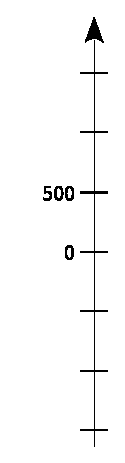
\includegraphics[width=1.2cm]{axe500}
  \end{minipage} \\
\end{exercice}


\begin{exercice}
On considère un immeuble comportant un rez-de-chaussée et cinq étages ainsi qu'un parking en sous-sol avec deux niveaux. 

Dessine le panneau de commandes de l'ascenseur de cet immeuble.
\end{exercice}


%%%%%%%%%%%%%%%%%%%%%%%%%%%%%%%%%%%%%%%%%%%%%%%%%%%%%%%%%%%%%%%%%%
\serie{Repérage sur une droite}

\begin{exercice}[Abscisses]
Pour chaque cas, lis puis écris les abscisses des points $A$, $B$, $C$, $D$ et $E$ :
\begin{enumerate}
  \item \textcolor{white}{Vilain truc pour forcer saut de ligne}

	\begin{center} 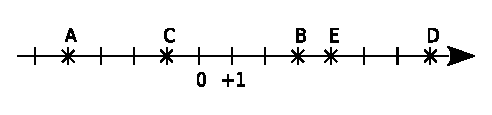
\includegraphics[width=7.4cm]{axeA} \end{center}



%%%%%%%%%%%%%%%%%%%%%%%%%%%%%Mise en page
%\vspace*{2em}
\newpage
%%%%%%%%%%%%%%%%%%%%%%%%%%%%%%%%%%%%%%%%%



  \item \textcolor{white}{Vilain truc pour forcer saut de ligne}

	\begin{center} 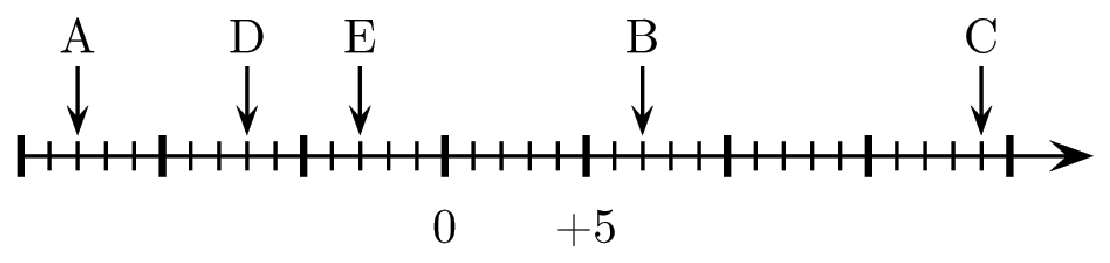
\includegraphics[width=7.4cm]{axeB} \end{center}
  \item \textcolor{white}{Vilain truc pour forcer saut de ligne}

	\begin{center} 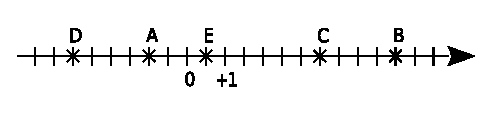
\includegraphics[width=7.4cm]{axeC} \end{center}
  \item \textcolor{white}{Vilain truc pour forcer saut de ligne}

	\begin{center} 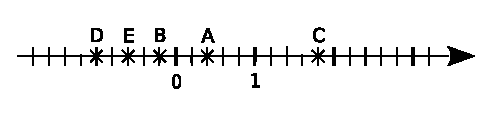
\includegraphics[width=7.4cm]{axeD} \end{center}
  \item \textcolor{white}{Vilain truc pour forcer saut de ligne}

	\begin{center} 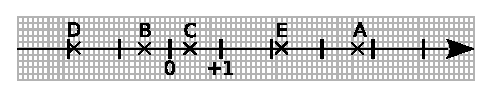
\includegraphics[width=7.4cm]{axeE} \end{center}
 \end{enumerate}
\end{exercice}


\begin{exercice}[Placements de points]
Reproduis les dessins de chaque droite graduée et place les points $A$, $B$, $C$, $D$ et $E$ d'abscisses respectives :

\begin{enumerate}
  \item \textcolor{white}{Vilain truc pour forcer saut de ligne}

	\begin{center} 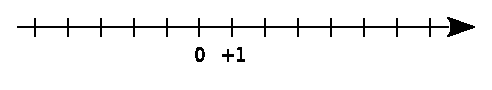
\includegraphics[width=7.4cm]{axeABCDE1} \end{center}
  
 $A(-1)$ ; $B(+4)$ ; $C(-3)$ ; $D(+3)$ ; $E(-5)$. \\[1em]
  \item \textcolor{white}{Vilain truc pour forcer saut de ligne}

	\begin{center} 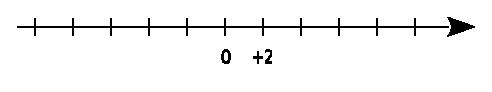
\includegraphics[width=7.4cm]{axeABCDE2} \end{center}
  
 $A(-2)$ ; $B(+4)$ ; $C(-6)$ ; $D(+8)$ ; $E(-8)$. \\[2em]
  \item \textcolor{white}{Vilain truc pour forcer saut de ligne}

	\begin{center} 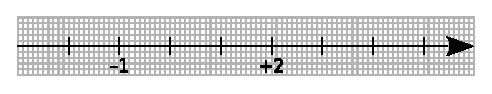
\includegraphics[width=7.4cm]{axeABCDE3} \end{center}
  
 $A(+4)$ ; $B(-0,5)$ ; $C(+0,8)$ ; $D(+3,4)$ ; $E(-2,1)$.
 \end{enumerate}
\end{exercice}


\begin{exercice}[Placements de points (bis)]
\begin{enumerate}
 \item Trace une droite graduée en prenant le centimètre comme unité.
 \item Place sur cette droite les points suivants : 
 
$A(-5)$ ; $B(+3)$ ; $C(+2)$ ; $D(-4)$ ; $E(+5)$ ;
 \item Place le milieu $L$ du segment $[AB]$. Lis puis écris l'abscisse du point $L$.
 \item Place le point $M$ tel que $C$ soit le milieu du segment $[EM]$. Lis et écris l'abscisse du point $M$.
 \end{enumerate}
\end{exercice}


\begin{exercice}
Trace une droite graduée et choisis une unité convenable pour placer les points suivants :
\begin{colitemize}{4}
 \item $A(52)$ ;
 \item $B(-36)$ ;
 \item $C(80)$ ;
 \item $D(-12)$.
 \end{colitemize}
\end{exercice}


\begin{exercice}[Histoires]
\begin{center} 
\includegraphics[width=7.4cm]{axe1000} \end{center}
Reproduis cette droite graduée pour que 5 cm correspondent à 1\,000 ans et place les événements suivants le plus précisément possible :
\begin{itemize}
 \item K : construction de la pyramide de Khéops, vers $\numprint{-2600}$ ;
 \item J : naissance de Jules César, en $-100$ ;
 \item N : début du Nouvel Empire, vers $\numprint{-1550}$ ;
 \item A : Alexandre le Grand envahit l'Égypte, vers $-350$ ;
 \item C : couronnement de Charlemagne, vers l'an $800$.
 \end{itemize}
\end{exercice}


\begin{exercice}
Réponds par Vrai ou Faux à chacune des affirmations suivantes et justifie la réponse :
\begin{center} 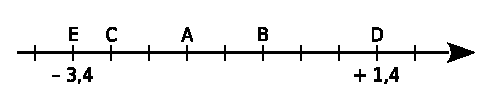
\includegraphics[width=7.4cm]{axeVrai} \end{center}
\begin{enumerate}
 \item Il y a exactement quatre entiers relatifs compris entre les abscisses des points $E$ et $D$ ;
 \item Le point $A$ a pour abscisse $-1,2$ ;
 \item L'abscisse de $B$ est positive ;
 \item L'abscisse de $C$ est $-2,8$ ;
 \item L'abscisse du milieu du segment $[AB]$ est un nombre entier relatif positif ;
 \item Exactement deux points ont une abscisse positive.
 \end{enumerate}
\end{exercice}


\begin{exercice}
Donne l'abscisse des points $A$, $B$ et $C$ :
\begin{center} 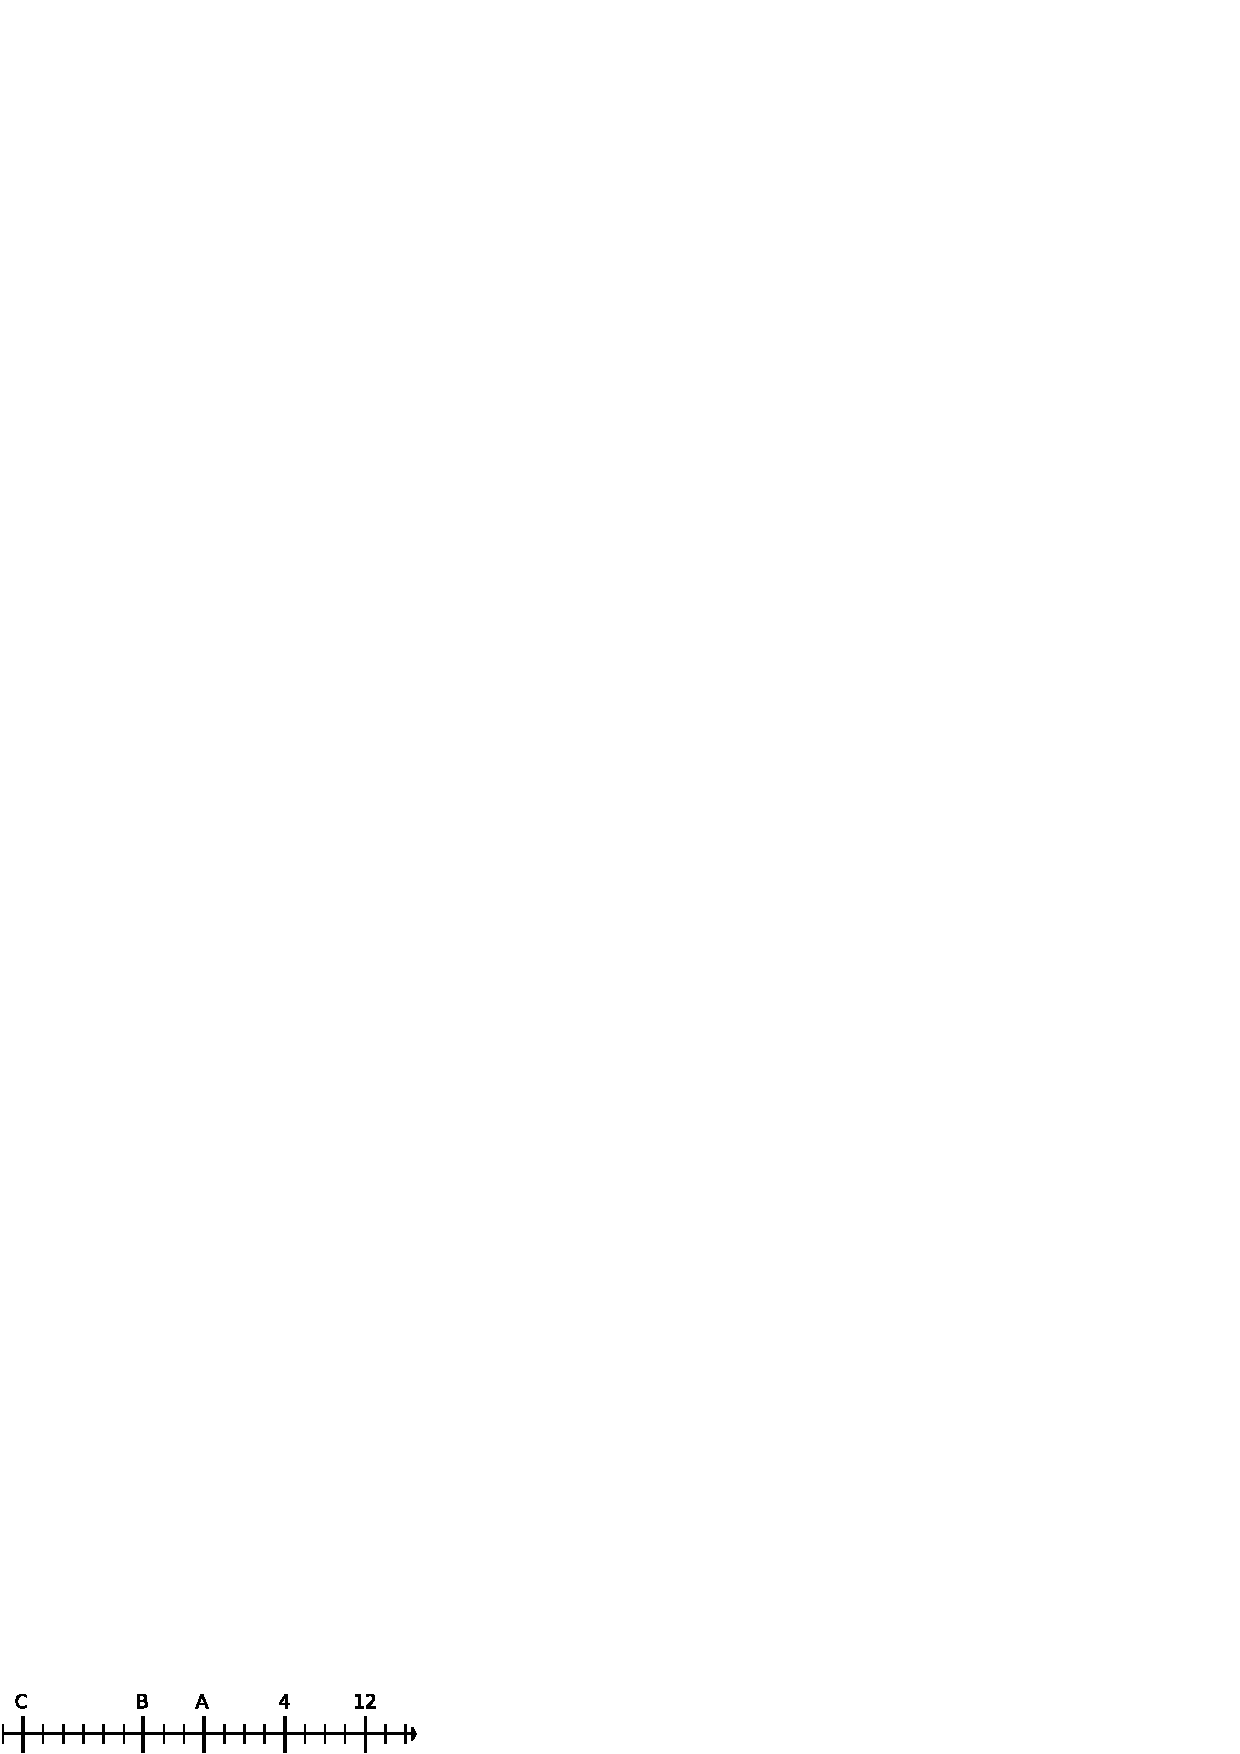
\includegraphics[width=6.7cm]{axeBAC} \end{center}

\dotfill

\dotfill
\end{exercice}


\begin{exercice}
Sur la droite ci-dessous, place les points $D(0,15)$, $E(- 0,1)$ et $F(0,55)$ :
\begin{center} 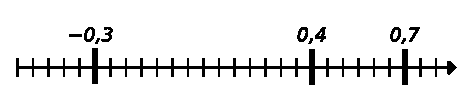
\includegraphics[width=7.1cm]{axe04}] \end{center}
\end{exercice}

\vspace*{1em}
%%%%%%%%%%%%%%%%%%%%%%%%%%%%%%%%%%%%%%%%%%%%%%%%%%%%%%%%%%%%%%%%%%
\serie{Repérage dans le plan}

\begin{exercice}[Signes des coordonnées]
\begin{minipage}[c]{0.3\linewidth}
Les axes de coordonnées d'un repère partagent le plan en quatre zones, notées $z_1$, $z_2$, $z_3$ et $z_4$.
 \end{minipage} \hfill%
 \begin{minipage}[c]{0.65\linewidth}
 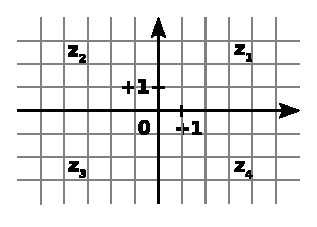
\includegraphics[width=4.6cm]{plan_colore}
  \end{minipage} \\[1em]
Pour chacune des zones, donne le signe de chacune des coordonnées (abscisse et ordonnée) d'un point de cette zone.
\end{exercice}


\begin{exercice}[Lecture de point]
Lis puis écris les coordonnées des points $A$, $B$, $C$, $D$, $E$, $F$, $G$ et $H$ ci-dessous :
\begin{center} 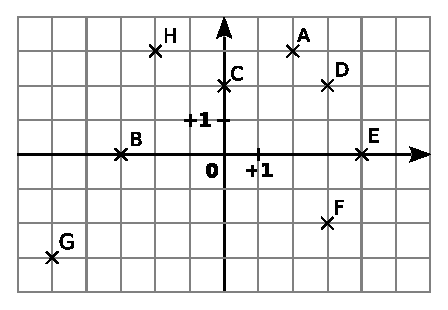
\includegraphics[width=6.7cm]{plan_blanc} \end{center}
\end{exercice}


\begin{exercice}
Lis puis écris les coordonnées des points $A$ à $K$ ci-dessous :
\begin{center} 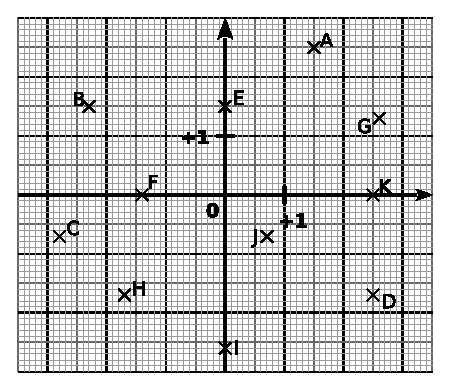
\includegraphics[width=6.7cm]{plan_noir} \end{center}
\end{exercice}


\begin{exercice}
Trace un repère d'unité 1 cm pour chaque axe puis place les 9 points suivants :
\begin{colitemize}{3}
 \item $P(+2 ; +5)$ ;
 \item $R(+2 ; -6)$ ;
 \item $S(-7 ; +4)$ ;
 \item $T(-5 ; -2)$ ;
 \item $U(0 ; -4)$ ;
 \item $V(+6 ; 0)$ ;
 \item $W(-3 ; -5)$ ;
 \item $X(+2 ; +6)$ ;
 \item $Y(+1 ; -5)$.
 \end{colitemize}
\end{exercice}


\begin{exercice}
Sur une feuille de papier millimétré, trace un repère d'unité 1 cm pour chaque axe puis place les points suivants :
\begin{colitemize}{2}
 \item $A(+1,5 ; -2,5)$ ;
 \item $B(-0,5 ; -1,5)$ ;
 \item $C(2,5 ; 1,5)$ ;
 \item $D(-3,5 ; +4,5)$ ;
 \item $E(-2,5 ; 0,5)$ ;
 \item $F(+4,5 ; 0)$ ;
 \item $G(-4,5 ; -3,5)$ ;
 \item $H(+4,5 ; -5,5)$ ;
 \item $I(0 ; -2,5)$ ;
 \item $J(-2,5 ; -1,5)$.
 \end{colitemize}
\end{exercice}


\begin{exercice}
Dans le repère ci-dessous, place les points suivants : 

$A(-2 ; 1)$ ; $B(-4 ; -3)$ ; $C(5 ; -1)$ ; $D(-5 ; 0)$ ; $E(0 ; -2)$.
\begin{center} 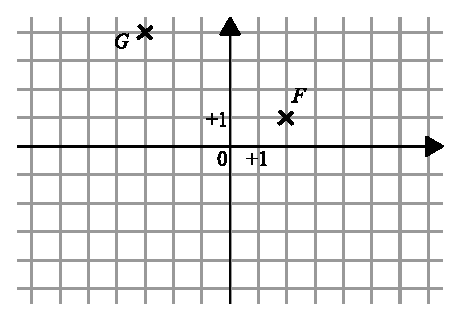
\includegraphics[width=6.9cm]{planGF} \end{center}
Donne ensuite les coordonnées des points $F$ et $G$.
\end{exercice}


%%%%%%%%%%%%%%%%%%%%%%%Mise en page
\newpage 
%%%%%%%%%%%%%%%%%%%%%%%%%%%%%%%%%%%

\begin{exercice}[Lapin et carotte]
\begin{center} 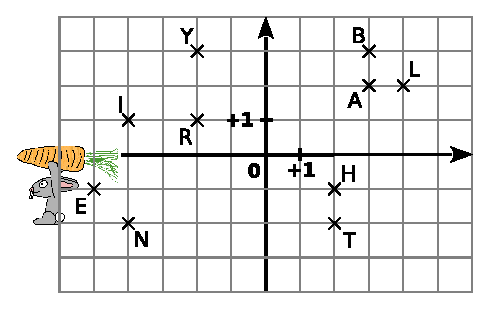
\includegraphics[width=7.2cm]{plan_carotte} \end{center}
Sur la grille ci-dessus, Monsieur Lapin aimerait dessiner l'itinéraire le conduisant à la carotte. Pour ce faire, il doit : 
\begin{itemize}
 \item Partir du point $L$ ; 
 \item Passer par tous les points de la figure une et une seule fois de telle sorte que deux points consécutifs aient une des deux coordonnées commune (abscisse ou ordonnée).
 \end{itemize}
 \begin{enumerate}
  \item Dessine le parcours sur la figure ;
  \item En écrivant dans l'ordre de passage chacune des lettres rencontrées, quel mot trouves-tu ?
  \end{enumerate}
\end{exercice}


%%%%%%%%%%%%%%%%%%%%%%%%%%%%%%%%%%%%%%%%%%%%%%%%%%%%%%%%%%%%%%%%%%

\serie{Comparer}


\begin{exercice}[Nombres relatifs et droite graduée]
\begin{enumerate}
 \item Trace une droite graduée en centimètre.
 \item Sur cette droite graduée, place les points suivants :

\begin{center} $A (+3)$ ; $B (-1)$ ; $C (-3)$ ; $D (+5)$ ; $E (-6)$. \end{center}
 \item En observant la droite graduée, range par ordre croissant les nombres suivants :
 
\begin{center} $+3$ ; $-1$ ; $-3$ ; $+5$ et $-6$.\end{center}
 \end{enumerate}
\end{exercice}


\begin{exercice}
Compare les nombres suivants :
\begin{colenumerate}{2}
 \item $-1$ et $+3$ ;
 \item $+4$ et $+6$ ;
 \item $-6$ et $-2$ ;
 \item $-2$ et $-4$ ;
 \item $-0$ et $+8$ ;
 \item $+3$ et $-4$ ;
 \item $+4$ et $-14$ ;
 \item $-12$ et $-18$ ;
 \item $-4$ et $0$ ;
 \item $-212$ et $+212$.
 \end{colenumerate}
 \end{exercice}
 
 
\begin{exercice}
Compare les nombres suivants :
\begin{enumerate}
 \item $-2,4$ et $-2,3$ \dotfill ;	
 \item $+3,6$ et $-6,3$ \dotfill ;
 \item $-11,3$ et $-9,7$ \dotfill	; 	
 \item $0$ et $+3,9$ \dotfill ; 	
 \item $-5,6$ et $-5,60$ \dotfill ;	 	
 \item $+9,6$ et $+6,9$ \dotfill	;	
 \item $+32,57$ et $+32,507$ \dotfill ;	 	
 \item $-125,64$ et $-125,064$ \dotfill ;	 	
 \item $-23,7$ et $+23,69$ \dotfill ;	
 \item $-15,878$ et $-15,8708$ \dotfill.
  \end{enumerate}
\end{exercice}
 
 
\begin{exercice}[Rangements]
Range par ordre croissant les nombres suivants :
\begin{enumerate}
 \item $+12$ ; $-2$ ; $+1$ ; $+13$ ; $-31$ ; $-11$ ; $-5$ ;
 \item $+15$ ; $-9$ ; $-8$ ; $+7$ ; $-3$ ; $-1$ ; $+6$ ;  $-4$ ; $-14$ ; $0$ ;
 \item $-25$ ; $+25,2$ ; $-5,2$ ; $+2,5$ ; $-3,2$ ; $+5,02$ ;
 \item $-100,3$ ; $-99,3$ ; $-100,03$ ; $-99,13$ ; $-9,3$.
 \end{enumerate}
\end{exercice}
        
    
\begin{exercice}[Rangements (bis)]
Range par ordre décroissant les nombres suivants :
\begin{enumerate}
 \item $+3$ ; $-15$ ; $+20$ ; $+15$ ; $-100$ ; $-25$ ; $+27$ :

 \dotfill
 
 \dotfill	
	
 \item $+12$ ; $-15$ ; $+17$ ; $+21$ ; $-13$ ; $-17$ ; $-5$ ; $-2$ ; $+3$ :
 
 \dotfill

 \dotfill	
	
 \item $+3,5$ ; $-20,39$ ; $-12,03$ ; $+5,6$ ; $-123,45$ :

 \dotfill
 
 \dotfill	
	
 \item $-7,001$ ; $-7,1$ ; $-7,71$ ; $-7,01$ ; $-7,2$ ; $-7,7$ :
 
 \dotfill
  
 \dotfill
 \end{enumerate}	
\end{exercice}


\begin{exercice}
Pour chaque nombre, complète par l'entier relatif qui suit ou qui précède :
\begin{colenumerate}{2}
 \item \ldots \ldots $< -4$ ;
 \item $-3 <$ \ldots \ldots ;
 \item $-12 >$ \ldots \ldots ;
 \item \ldots \ldots $> -15$ ;
 \item \ldots \ldots $< -35$ ;
 \item \ldots \ldots $< +125$. 
 \end{colenumerate}	
\end{exercice}


\begin{exercice}
Pour chaque nombre, recopie puis complète par l'entier relatif qui suit ou qui précède :
\begin{colenumerate}{2}
 \item \ldots \ldots $< -2,3$ ;
 \item $-1,1 <$ \ldots \ldots ;
 \item \ldots \ldots $> +3,2$ ;
 \item $+5,71 >$ \ldots \ldots ;
 \item \ldots \ldots $> -17,71$ ;
 \item $-114,5 >$ \ldots \ldots ;
 \end{colenumerate}	
\end{exercice}



%%%%%%%%%%%%%%%%%%%%%%%Mise en page
\newpage 
%%%%%%%%%%%%%%%%%%%%%%%%%%%%%%%%%%%


\begin{exercice}
Complète en intercalant un nombre entre les deux nombres proposés :
\begin{enumerate}
 \item $-2 > \ldots \ldots > -4$ ;
 \item $+5 < \ldots \ldots < +6$ ;
 \item $-14 > \ldots \ldots > -17$ ;
 \item $0 > \ldots \ldots > -2$ ;
 \item $+14 < \ldots \ldots < +16$ ;
 \item $-1,44 < \ldots \ldots < +0,71$ ;
 \item $-17,304 > \ldots \ldots > -17,34$ ;
 \item $-132,247 < \ldots \ldots < -132,24$.
 \end{enumerate}
\end{exercice}


\begin{exercice}
Complète par $<$ ou $>$ ou $=$ :
\begin{colitemize}{2}
 \item $+5,34 \ldots \ldots +3,54$ ;
 \item $-9,27 \ldots \ldots -9,272$ ;
 \item $0,05 \ldots \ldots 1$ ;
 \item $+8,64 \ldots \ldots -8,64$ ;
 \item $-8,51 \ldots \ldots -8,5$ ;
 \item $-19,2 \ldots \ldots +9,2$ ;
 \item $11,9 \ldots \ldots +11,9$ ;
 \item $-14,39 \ldots \ldots -14,4$ ;
 \item $-3,14 \ldots \ldots -1,732$ ;
 \item $-0,99 \ldots \ldots -0.909$.
 \end{colitemize}
\end{exercice}


\begin{exercice}
Range par ordre croissant les nombres suivants : \\[0.5em]
$+5,0$ ; $+2,7$ ; $-2,6$ ; $-3,1$ ; $+5,1$ ; $-1,7$ ; $-2,06$ ; $-0,2$ :

 \dotfill

 \dotfill
\end{exercice}


\begin{exercice}
Range par ordre décroissant les nombres suivants : \\[0.5em]
$-10,6$ ; $+14,52$ ; $-8,31$ ; $+4,2$ ; $+14,05$ ; $-14,5$ ; $-8,003$ :

 \dotfill

 \dotfill
\end{exercice}


%%%%%%%%%%%%%%%%%%%%%%%Mise en page
\vspace{1cm}
%%%%%%%%%%%%%%%%%%%%%%%%%%%%%%%%%%%


\begin{exercice}
Encadre chaque expression par deux nombres entiers consécutifs :
\begin{colitemize}{2}
 \item $\ldots < -2,3 < \ldots$ ;
 \item $\ldots < +4,2 < \ldots$ ;
 \item $\ldots < -15,11 < \ldots$ ;
 \item $\ldots < -0,14 < \ldots$ ;
 \item $\ldots < +0,14 < \ldots$ ;
 \item $\ldots < -0,98 < \ldots$ ;
 \item $\ldots < -12,7 < \ldots$ ;
 \item $\ldots < -0,003 < \ldots$ .
 \end{colitemize}
\end{exercice}


\begin{exercice}[Bulletin météo]
Voici quelques températures relevées à différents moments de la journée dans plusieurs villes de Suisse : \\[0.5em]
\renewcommand*\tabularxcolumn[1]{>{\centering\arraybackslash}m{#1}} %permet de centrer le texte dans les cellules
\begin{cltableau}{\linewidth}{4}
 \hline
 & Matin ($^\circ$C) & Midi ($^\circ$C) & Soir ($^\circ$C) \\\hline
 Lausanne & $-4$ & $+1$ & $-1$ \\\hline
 Delémont & $+2$ & $+4$ & $+3$ \\\hline
 Sion & $+5$ & $+9$ & $+6$ \\\hline
 Neuchâtel & $-10$ & $-6$ & $-7$ \\\hline
 Fribourg & $-2$ & $0$ & $-3$ \\\hline
 Berne & $0$ & $+2$ & $-2$ \\\hline
 Genève & $+4$ & $+7$ & $+2$ \\\hline
 \end{cltableau}
 \vspace{0.3cm}
\begin{enumerate}
 \item Range ces villes dans l'ordre croissant de  leur température du matin ;
 \item Range ces villes dans l'ordre décroissant de  leur température du soir ;
 \item Calcule la température moyenne de la journée pour Delémont, Sion et Genève.
 \end{enumerate}
\end{exercice}


\end{colonne*exercice}


\exercicesappr
\begin{colonne*exercice}
\begin{exercice}[Histoire]
Classe les dates des événements suivants par ordre chronologique :
\begin{itemize}
 \item Signature du pacte fédéral d'alliance perpétuelle entre les communautés d'Uri, Schwytz et Nidwald : $\numprint{1291}$ ;
 \item La mort de Toutankhamon : $\numprint{-1327}$ ;
 \item L'éruption du Vésuve qui ensevelit Pompéi sous les cendres : $79$ ;
 \item La défaite d'Alésia : $52$ av. J.-C. ;
 \item La mort de Léonard de Vinci : $\numprint{1519}$ ;
 \item La naissance de Jules César : $100$ av. J.-C. ;
 \item Le début de la guerre de $100$ ans : $\numprint{1337}$ ;
 \item La naissance de Socrate : $470$ av. J.-C. ;
 \item Ta date de naissance.
 \end{itemize}
\end{exercice}


\begin{exercice}[Géographie]
Complète le tableau en recherchant les altitudes maximales et les profondeurs (altitudes minimales) :\\[0.5em]
\begin{cltableau}{\linewidth}{3}
 \hline
 & Sommets, altitude maximale & Profondeurs, altitude minimale \\\hline
 Afrique & Kilimandjaro & Lac Assal\\
 & & \\\hline
 Europe & Elbrouz & Mer Caspienne \\
 & & \\\hline
 Amérique du sud & Aconcagua & Rio Negro \\\hline
 Asie & Everest & Mer Morte \\
 & & \\\hline
 Océan pacifique & Mauna Kea & La fosse des Mariannes \\
 & & \\\hline
 \end{cltableau}
  \vspace{0.3cm}
\begin{enumerate}
 \item Quel est le sommet le plus haut ?
 \item La mer Caspienne est-elle plus profonde que le Rio Negro ?
 \item En Afrique, combien de mètres séparent le point le plus profond du lac Assal et le sommet du Kilimandjaro ?
 \item Un poisson se trouve tout au fond de la mer morte. À quelle distance se trouve-t-il de la surface de l’eau ?
 \end{enumerate}
\end{exercice}


\begin{exercice}[Repères]
Dans chaque cas, trace un repère en choisissant judicieusement l'unité pour pouvoir placer tous les points :
\begin{enumerate}
 \item $A(-3 ; 3)$ ; $B(1 ; 4)$ et $C(5 ; 2)$ ; 
 \item $D(-13 ; 8)$ ; $E(25 ; 14)$ et $F(-35 ; 22)$ ;
 \item $G(-83 ; -8)$ ; $H(72 ; -55)$ et $I(-15 ; 32)$.
 \end{enumerate}
\end{exercice}


\begin{exercice}[Coordonnées mystères]
\begin{enumerate}
 \item Construis un repère et places-y les points $A$, $B$, $C$, $D$, $E$ et $F$ sachant que :
 \begin{itemize}
  \item Les valeurs des coordonnées des six points sont :
$0$ ; $0$ ; $3$ ; $4$ ; $-2$ ; $2$ ; $-4$ ; $1$ ; $-1$ ; $3$ ; $-1$ et $-2$ ;
  \item Les ordonnées des six points sont toutes différentes et si on range les points dans l'ordre décroissant de leurs ordonnées, on obtient : $E$, $B$, $F$, $C$, $A$ et $D$ ;
  \item Les abscisses de tous les points sauf $D$ sont différentes et si on range les points dans l'ordre croissant de leurs abscisses, on obtient : $F$, $B$, $A$, $E$ et $C$ ;
  \item Le point $E$ est sur l'axe des ordonnées ;
  \item L'ordonnée de $E$ est l'opposé de l'abscisse de $F$ ;
  \item Le point $C$ est sur l'axe des abscisses à une distance de 3 de l'origine ;
  \item Les deux coordonnées du point $B$ sont opposées.
  \end{itemize}
 \item Que dire de la droite $(CD)$ ? Justifie ta réponse.
 \end{enumerate}
\end{exercice}




\end{colonne*exercice}

\connaissances


\QCMautoevaluation{Pour chaque question, plusieurs réponses sont % enlever le lien internet
  proposées.  Déterminer celles qui sont correctes.}

\begin{QCM}
  \begin{GroupeQCM}
    \begin{exercice}
      Le nombre $-4$ est \ldots
      \begin{ChoixQCM}{4}
      \item positif
      \item négatif
      \item l'opposé de $4$
      \item la valeur absolue de $4$
      \end{ChoixQCM}
\begin{corrige}
     \reponseQCM{bc} 
   \end{corrige}
    \end{exercice}
    
    
    \begin{exercice}
      Le nombre 3 est \ldots
      \begin{ChoixQCM}{4}
      \item positif
      \item négatif
      \item ni positif ni négatif
      \item l'opposé de $-3$
      \end{ChoixQCM}
\begin{corrige}
     \reponseQCM{ad} 
   \end{corrige}
    \end{exercice}


    \begin{exercice}
      La valeur absolue de $-10$ est \ldots
      \begin{ChoixQCM}{4}
      \item positive
      \item négative
      \item $-10$
      \item $10$
      \end{ChoixQCM}
\begin{corrige}
     \reponseQCM{ad} 
   \end{corrige}
    \end{exercice}


    \begin{exercice}
      L'abscisse de $A$ est \ldots 
\vspace{-2em}
\begin{center}  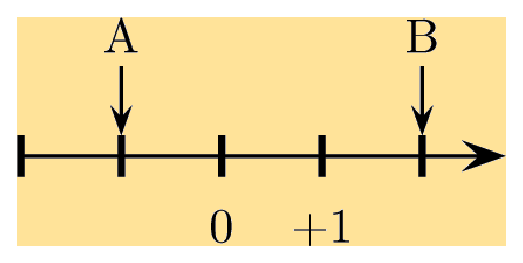
\includegraphics[width=2.6cm]{axeAB} \end{center}

      \begin{ChoixQCM}{4}
      \item $-1$
      \item $-2$
      \item positive
      \item négative
      \end{ChoixQCM}
\begin{corrige}
     \reponseQCM{ad} 
   \end{corrige}
    \end{exercice}
    
    
     \begin{exercice}
      Sur la droite précédente, l'abscisse de $B$ est \ldots
      \begin{ChoixQCM}{4}
      \item l'opposé de celle de $A$
      \item la valeur absolue de $-2$
      \item la valeur absolue de celle de $A$
      \item positive
      \end{ChoixQCM}
\begin{corrige}
     \reponseQCM{bd} 
   \end{corrige}
    \end{exercice}
    

    \begin{exercice}
      L'abscisse de $B$ est \ldots \hspace{0.4em} l'abscisse de $A$. 
      
\vspace{-2em}
\begin{center} 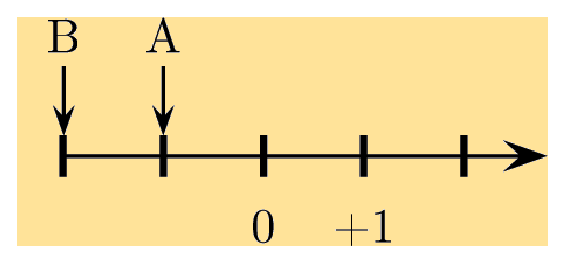
\includegraphics[width=2.6cm]{axeBA} \end{center}

      \begin{ChoixQCM}{4}
      \item plus grande que
      \item plus petite que
      \item $>$
      \item $<$
      \end{ChoixQCM}
\begin{corrige}
     \reponseQCM{bd} 
   \end{corrige}
    \end{exercice}
    
 
     \begin{exercice}
      $-3$ est \ldots 3
      \begin{ChoixQCM}{4}
      \item plus grand que
      \item plus petit que
      \item la valeur absolue de
      \item l'opposé de
      \end{ChoixQCM}
\begin{corrige}
     \reponseQCM{bd} 
   \end{corrige}
    \end{exercice}
 \end{GroupeQCM}
\end{QCM}
 
 
\begin{QCM}
  \begin{GroupeQCM}   
    \begin{exercice}
      $-5$ \ldots $-7$
      \begin{ChoixQCM}{4}
      \item $>$
      \item $<$
      \end{ChoixQCM}
\begin{corrige}
     \reponseQCM{a}
   \end{corrige}
    \end{exercice}
    

    
    \begin{exercice}
      $-30$ \ldots $-35$
      \begin{ChoixQCM}{4}
      \item $>$
      \item $<$
      \end{ChoixQCM}
\begin{corrige}
     \reponseQCM{a}
   \end{corrige}
    \end{exercice}
    \begin{exercice}
      $-1,95$ \ldots $-1,94$
      \begin{ChoixQCM}{4}
      \item $>$
      \item $<$
      \end{ChoixQCM}
\begin{corrige}
     \reponseQCM{b}
   \end{corrige}
    \end{exercice}
    
    
    \begin{exercice}
      $-2,04$ \ldots $-2,048$
      \begin{ChoixQCM}{4}
      \item $>$
      \item $<$
      \end{ChoixQCM}
\begin{corrige}
     \reponseQCM{a}
   \end{corrige}
    \end{exercice} 

\end{GroupeQCM}
\end{QCM}

  


\TravauxPratiques % pour nous "travailler en groupe"

\begin{TP}[Les vacances de Polo]

Ci-dessous un repère quadrille la carte de France.

\begin{center} 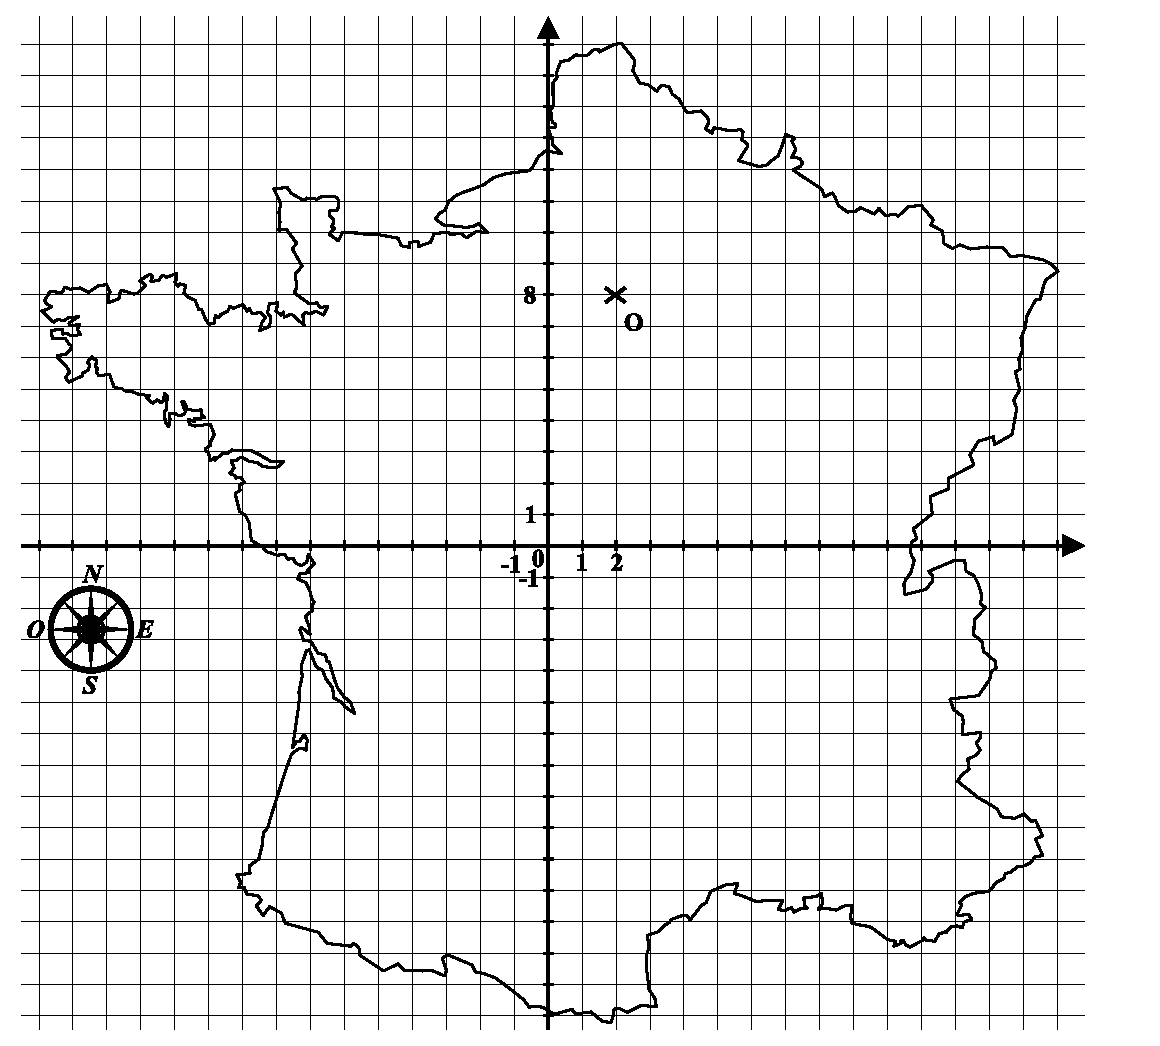
\includegraphics[width=12cm]{carteNOES} \end{center}

\begin{enumerate}
 \item Déterminez les coordonnées des points $A$, $B$, $C$, $D$, $E$, $F$, $G$, $H$, $I$, $J$, $K$, $L$, $M$, $N$, $O$, $P$, $R$, $S$ et $T$ sachant que :
 \begin{itemize}
  \item $A$ a pour abscisse $5$ et pour ordonnée $10$ ;
  \item $B$ a pour abscisse $-3$ et pour ordonnée $11$ ;
  \item L'ordonnée de $C$ est $-11$ et son abscisse est $5$ ;
  \item $D(-7 ; -1)$ et $E(3,5 ; 0)$ ;
  \item $F$ a pour ordonnée $-10$ et est aussi à l'Ouest que possible ;
  \item $G(-14 ; 7,5)$ ;
  \item $H$ a la même abscisse que $D$ et la même ordonnée que $G$ ;
  \item $I$ ne peut pas être plus au Nord ;
  \item La droite $(IB)$ (droite passant par les points $I$ et $B$) coupe l'axe des ordonnées au point $J$ ;
  \item Le point $K$ est le symétrique de $J$ par rapport à l'axe des abscisses ;
  \item $L$ est au bord de la mer et a la même ordonnée que $K$ ;
  \item $M$ a pour ordonnée $7$, et est aussi à l'Est que possible ;
  \item L'abscisse de $N$ est égale à l'ordonnée de $A$, et son ordonnée est l'opposée de l'abscisse de $C$ ;
  \item $O$ se lit sur la carte ;
  \item $P$ est à l'intersection des droites $(MN)$ et $(LC)$ ;
  \item $R$ est sur la droite $(KG)$, et son abscisse est égale à son ordonnée ;
  \item $S$ a pour abscisse $7$ et est sur la droite $(PR)$ ;
  \item $T$ et $S$ ont la même ordonnée, mais l'abscisse de $T$ est l'opposée de l'abscisse de $S$.
  \end{itemize}
 \item Chaque point sur la carte correspond à une des villes suivantes :
  \begin{colitemize}{3}
   \item Paris ;
   \item Etretat ;
   \item Moulins ;
   \item Lyon ;
   \item Annecy ;
   \item Montpellier ;
   \item Bordeaux ;
   \item Le Mont Saint-Michel ;
   \item La Rochelle ;
   \item Grenoble ;
   \item Perpignan ;
   \item Royan ;
   \item Brest ;
   \item Le Touquet ;
   \item Dunkerque ;
   \item Tarascon-sur-Ariège ;
   \item Reims ;
   \item Strasbourg ;
   \item Biarritz.
     \end{colitemize}
   À l’aide de votre atlas et de la liste ci-dessus, retrouvez et écrivez pour chaque point la ville qui lui correspond.
 \item Sachant que Polo se rend au point $T$, où ira-t-il en vacances cette année?
 \item Parmi les villes que vous venez de placer, la distance entre la ville la plus au Nord de la carte et celle la plus au Sud située en bord de mer correspond environ à 1000 km.
 
Sachant que Polo part de Reims, calculez approximativement la distance (en kilomètres et en ligne droite) qui sépare Polo de son lieu de vacances ?
  \end{enumerate}
\end{TP}

%%%%%%%%%%%%%%%%%%%%%%%%%%%%%%%%%%%%%%%%%%%%%%%%%%%%%%%%%%%%%%%%%%%

\begin{TP}[Bataille navale]

\begin{enumerate}
 \item Chaque groupe trace un repère d'unité 1 cm pour chaque axe. Les graduations pour l'axe des abscisses et celui des ordonnées vont de $- 5$ à $+ 5$.
 \item Chaque équipe dessine les bateaux ci-dessous dans le repère, horizontalement ou verticalement. Les croix doivent être sur des coordonnées entières du repère. \\[0.5em]
\begin{tabularx}{\linewidth}{XX}
 
 Yawl & 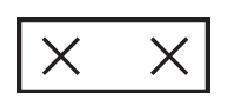
\includegraphics[width=1.3cm]{2X} \\
 Mayflower & 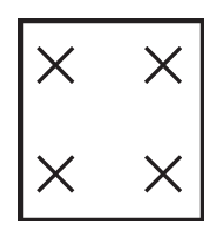
\includegraphics[width=1.4cm]{4X} \\
 Titanic & 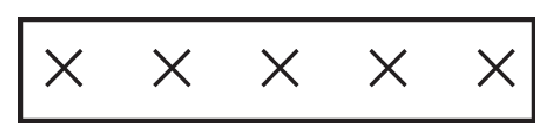
\includegraphics[width=3.5cm]{5X} \\
 USS Gerald R.Ford & 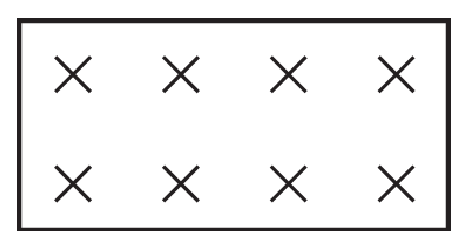
\includegraphics[width=3.5cm]{8X} \\
 \end{tabularx}
 \vspace{0.3cm}
 \item Alternativement chaque équipe répond par raté, touché ou coulé à ses attaquants. L'équipe gagne une fois que tous les bateaux des adversaires sont coulés.
 \end{enumerate}
 
\end{TP}



\pagebreak

\recreation
\begin{enigme}[Puce « olympique »]

Lorsqu'elle utilise sa patte gauche seule, elle fait des bonds de 6 cm.

Lorsqu'elle utilise sa patte droite seule, elle fait des bonds de 4 cm.

Et lorsqu'elle saute « à pattes jointes », elle fait des bonds de 34 cm !

Quel est le nombre \underline{minimum} de bonds qu'elle doit réaliser pour parcourir exactement 20 m ?

Même question avec 35 m.
 
 \end{enigme}
 
 \vspace*{2em}
 
%%%%%%%%%%%%%%%%%%%%%%%%%%%%%%%%%%%%%%%%%%%%%%%%%%%%%%%%%%%%%%%%%%%%%

\begin{enigme}[Abracadabra]

Un magicien donne la formule magique à son apprenti.

« Voici la formule magique, elle est formée d'une infinité de séquences $AB$ et $BA$. Lorsque tu l'auras recopiée, tu seras mon égal ».

L'apprenti, pour gagner du temps, remplace chaque bloc $AB$ par la lettre $A$ et chaque bloc $BA$ par la lettre $B$, et, oh stupeur ! La formule magique reste inchangée !

Quelles sont les \numprint{2002}\up{ème}, \numprint{2003}\up{ème}, \numprint{2004}\up{ème}, \numprint{2005}\up{ème}, \numprint{2006}\up{ème}, \numprint{2007}\up{ème} et \numprint{2008}\up{ème} lettres de la formule magique ?

\end{enigme} 



